\documentclass[9pt]{IEEEtran}

\usepackage[english]{babel}
\usepackage{graphicx}
\usepackage{epstopdf}
\usepackage{fancyhdr}
\usepackage{amsmath}
\usepackage{amsthm}
\usepackage{amssymb}
\usepackage{url}
\usepackage{array}
\usepackage{textcomp}
\usepackage{listings}
\usepackage{hyperref}
\usepackage{xcolor}
\usepackage{colortbl}
\usepackage{float}
\usepackage{gensymb}
\usepackage{longtable}
\usepackage{supertabular}
\usepackage{multicol}

\usepackage[utf8x]{inputenc}

\usepackage[T1]{fontenc}
\usepackage{lmodern}
\input{glyphtounicode}
\pdfgentounicode=1

\graphicspath{{./figures/}}
\DeclareGraphicsExtensions{.pdf,.png,.jpg,.eps}

% correct bad hyphenation here
\hyphenation{op-tical net-works semi-conduc-tor trig-gs}

% ============================================================================================

\title{\vspace{0ex}
Mathematics 2, Part 4, Homework 1}


% ============================================================================================

\begin{document}

\maketitle
\section{Nelder-Mead implementation}
\subsection*{2-D implementation}
Firstly we implemented the two dimensional version of the Nelder-Mead method
 and tested it on a simple function: 
 \[f(x, y) = x^2 + y^2 \]

 On Figure~\ref{fig:nelder_2d} we can see the convergence of the best points using 
 the 2-d implementation of the method. 

\begin{figure}[h]
    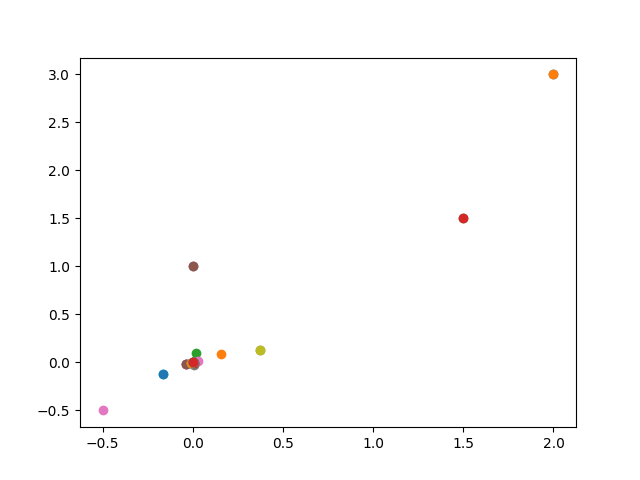
\includegraphics[width=\columnwidth]{convergence1.png}
    \caption{Convergence of the best points on a simple function for a 2-d implemntation 
    of the Nelder-Mead method}
    \label{fig:nelder_2d}
\end{figure}

\subsection*{Implementation for arbitrary dimensions}
Next, we implemented Nelder-Mead for arbitrary dimensions and tested it on the 
same function. On Figure~\ref{fig:nelder} We can see that, when using the same starting points, we achieve 
the same convergence as for the previous implemtation. Note that, we require the
 user the specify one starting point for this implementation. The other starting 
 points are determined by taking the first starting point and adding a constant \textit{r}
 (which is another parameter for the method) to a different dimension each time (for each 
 different point). 

\begin{figure}[h]
    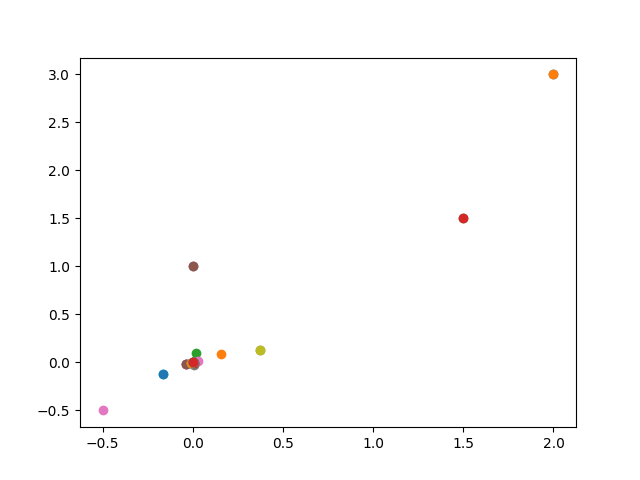
\includegraphics[width=\columnwidth]{convergence1.png}
    \caption{Convergence of the best points on a simple function 
    for the arbitrary dimensional implementation of the Nelder-Mead method}
    \label{fig:nelder}
\end{figure}

\section{Comparison of Nelder-Mead with descent methods}
We compared the implemented method with the previously implemented descent 
methods on 3 different functions. To compare the implemented method with the descent 
methods, we used the results from the second homework, where we looked at the number 
of steps needed to reach convergence, where our convergence condition was 
where the difference in our
positions (of consequitive steps) is small enough. We add our results for 
the Nelder-Mead method to our results from the second homework. For each function 
we used both starting points given in the second homework
 and we evaluate the Nelder-Mead method with three 
different \textit{r}-s, those being 1,2 and 5.

\subsection*{Function 1}
The first function is given as:
\[
f_1(x) = (x_0 - x_2)^2 + (2x_1 + x_2)^2 + (4x_0 - 2x_1 + x_2)^2 + x_0 + x_1
\]
For this function we used the starting points of (0, 0, 0) and (1, 1, 0).
We can see the results in Table~\ref{tab:f1}. Note that here and on the other tables
S1 and S2 denote the first and second starting points and f denotes the value of 
the function in the final point. We can see that 
Nelder-Mead was outperformed by second degree methods (and their aproximations) and 
Adagrad, however it outperformed the basic gradient descent and its Polyak and 
Nesterov modifications. Changing \textit{r} did not influence the result much 
for this function.

\begin{table}[h!]
    \centering
    \begin{tabular}{|c|c|c|c|c|}
        \hline
        \textbf{Method} & \textbf{S1: f} & \textbf{S1: Stps} & \textbf{S2: f} & \textbf{S2: Stps} \\ \hline
        GD         & -0.1979  & 3142  & -0.1979  & 3611 \\ \hline
        Polyak     & -0.1979  & 1561  & -0.1979  & 1794 \\ \hline
        Nesterov   & -0.1979  & 1565  & -0.1979  & 1798 \\ \hline
        AdaGrad    & -0.1979  & 101   & -0.1979  & 79   \\ \hline
        Newton     & -0.1979  & 1     & -0.1979  & 1    \\ \hline
        Bfgs       & -0.1979  & 20    & -0.1979  & 22   \\ \hline
        L-Bfgs    & -0.1979  & 8     & -0.1979  & 11   \\ \hline
        NM, r=1 & -0.1979 & 126 & -0.1979 & 141  \\ \hline
        NM, r=2 & -0.1979 & 136 & -0.1979 & 131  \\ \hline
        NM, r=5 & -0.1979 & 138 & -0.1979 & 132  \\ \hline

    \end{tabular}
    \vspace{3pt}
    \caption{Comparison of the Nelder-Mead method with descent methods on the first 
    function}
    \label{tab:f1}
\end{table}

\subsection*{Function 2}
Next, we used the function:
\[
f_2(x) = (x_1 - 1)^2 + (x_2 - 1)^2 + 100(x_2 - x_1^2)^2 + 100(x_3 - x_2^2)^2
\]
Here, the starting poins were (1.2, 1.2, 1.2) and (-1, 1.2, 1.2). 
We can see the comparison in Table~\ref{tab:f2}. Note that here the descent methods 
were only allowed 2 second of runtime, since that was the task in the second homework, however the 
Nelder-Mead method finished much faster, so this criteria still held.
We can quickly see that with and appropriate choice of \textit{r} the 
Nelder-Mead method performs really nicely even in comparison to second degree 
methods, however when choosing 
an \textit{r} that is too large, the method does not converge properly.



\begin{table}[h]
    \centering
    \begin{tabular}{|c|c|c|c|c|}
        \hline
        \textbf{Method} & \textbf{S1: f} & \textbf{S1: Stps} & \textbf{S2: f} & \textbf{S2: Stps} \\ \hline
        GD       & $3.27 \times 10^{-8}$ & 24966  & $3.26 \times 10^{-8}$  & 30730 \\ \hline
        Polyak   & $3.26 \times 10^{-8}$ & 12430 & $3.26 \times 10^{-8}$   & 15350 \\ \hline
        Nesterov & $3.26 \times 10^{-8}$& 14134   & $3.26 \times 10^{-8}$  & 13784 \\ \hline
        AdaGrad  & $3.60 \times 10^{-9}$  & 13498   & $4.62 \times 10^{-9}$& 15915 \\ \hline
        Newton   & $1.84 \times 10^{-1}$ & 67541  & $3.83\times 10^{-1}$  & 66239 \\ \hline
        Bfgs     & $1.93 \times 10^{-15}$& 319 & $4.70 \times 10^{-16}$     & 188   \\ \hline
        L-Bfgs   & $5.16 \times 10^{-11}$  & 369& $2.25 \times 10^{-8}$    & 509   \\ \hline
        NM, r=1 & $6.33 \times 10^{-15}$  & 178 & $3.46 \times 10^{-14}$ & 1294  \\ \hline
        NM, r=2 & $1.09 \times 10^{-13}$  & 169 & 0.24 & 113 \\ \hline
        NM, r=5 & 7.33 & 123 & 2.32 & 102  \\ \hline
    
    \end{tabular}
    \caption{Comparison of the Nelder-Mead method with descent methods on the second 
    function}
    \label{tab:f2}
\end{table}


\subsection*{Function 3}
The last function was given as: 
\[
f_3(x) = (1.5 - x_1 + x_1 x_2)^2 + (2.25 - x_1 + x_1 x_2^2)^2 + (2.625 - x_1 + x_1 x_2^3)^2
\]
The starting points were (1, 1) and (4.5, 4.5). We can see the comparison on 
Table~\ref{tab:f3}. Here, we can see that for the second starting point, all the 
other methods fail to reach the optimum, while the Nelder-Mead method finds it 
really quickly, if we choose the correct \textit{r}. 

\begin{table}[h]
    \centering
    \begin{tabular}{|c|c|c|c|c|}
        \hline
        \textbf{Method} & \textbf{S1: f} & \textbf{S1: Stps} & \textbf{S2: f} & \textbf{S2: Stps} \\ \hline
        GD       & $1.65\times10^{-8}$  & 23234  & $\text{nan}$          & 100000 \\ \hline
        Polyak   & $1.65\times10^{-8}$  & 11607  & $\text{nan}$          & 100000 \\ \hline
        Nesterov & $1.65\times10^{-8}$  & 11617  & $\text{nan}$          & 100000 \\ \hline
        AdaGrad  & $1.0\times10^{-12}$ & 318    & $0.22$            & 27017  \\ \hline
        Newton   & $14.20$             & 1      & $14.20$           & 12     \\ \hline
        BFGS     & $4.66\times10^{-18}$ & 31     & $\text{nan}$          & 71794  \\ \hline
        L-BFGS   & $1.18\times10^{-14}$ & 29     & $1.74\times10^{5}$ & 3      \\ \hline
        NM, r=1 & $6.58 \times 10^{-15}$  & 65 & 0.125 & 48 \\ \hline
        NM, r=2 & $4.87 \times 10^{-15}$  & 61 & $1.37 \times 10^{-14}$ & 91 \\ \hline
        NM, r=5 & $1.76 \times 10^{-15}$  & 73 & $5.44 \times 10^{-14}$ & 81 \\ \hline
    \end{tabular}
        \caption{Comparison of the Nelder-Mead method with descent methods on the third
    function}
    \label{tab:f3}
\end{table}

\section{Finding minima of blackbox functions}
In this section, we use the method on the 3 provided blackbox functions. Note 
that the student ID used was 63240454. We provide the achieved minima on 
Table~\ref{tab:bb}, where we can oberve the points, as well as the functions 
evaluated at those points.

\begin{table}[h]
    \centering
    \begin{tabular}{|c|c|c|}
        \hline
      f & Point & Evaluation \\\hline
    1 & [0.36444539 0.42364448 0.40423644] & 0.454042360000001 \\\hline
    2 & [0.40423663 0.42364442 0.36444534] & 0.454042360000015 \\\hline
    3 & [0.42364444 0.40423646 0.36444535] & 0.454042360000001 \\\hline

    \end{tabular}
    \label{tab:bb}
    \vspace{3pt}
    \caption{Minima of blackbox functions}
\end{table}

\section{Jeklo Ruše revisited}
In this section we used the provided recipe to solve the Jeklo Ruše problem. We achieved that 
by using the sympy python equation solver. We firstly checked all possible combination of 
using the 2 equalities and then for each solution checked if the other two inequalities 
were still satisfied under those solutions. We solved that by producing 180 pitchforks and 
60 shovels we can achieve the highest profit of 660 Euros. 

\end{document}
